\documentclass[11pt]{article}

\usepackage{minted}
\usepackage[scale=1]{ccicons}
\usepackage{metalogo}
\usepackage{xcolor,colortbl}
\usepackage{multicol,multirow,booktabs}
\usepackage{graphicx}
\usepackage{bm}
\usepackage{fontawesome}
\usepackage{exsheets}
\usepackage[paper=a4paper, headheight=110pt,showframe=false, 
            layoutvoffset=2em,
            bottom=2cm, top=3.5cm]{geometry}
\usepackage[spanish, es-nodecimaldot]{babel}
\usepackage[babel]{microtype}
\usepackage{hyperref}
\usepackage{amsmath}
\usepackage{mismath}
\usepackage{gensymb,amssymb}
\setlength{\parindent}{3em}
\setlength{\parskip}{1em} 
\usepackage[shortlabels]{enumitem}
\usepackage{subcaption}
\usepackage{wrapfig}
%\usepackage{mathspec}
\usepackage{unicode-math}


% Fonts can be customized here.
\defaultfontfeatures{Mapping=tex-text}
\setmainfont [Ligatures={Common}]{Linux Libertine O}
\setmonofont[Scale=0.9]{Linux Libertine Mono O}
%\usepackage[svgnames]{xcolor} % Gestión de colores
\usepackage{hyperref}
\hypersetup{
  colorlinks=true, linktocpage=true, pdfstartpage=3, pdfstartview=FitV,%
  breaklinks=true, pageanchor=true,%
  pdfpagemode=UseNone, %
  plainpages=false, bookmarksnumbered, bookmarksopen=true, bookmarksopenlevel=1,%
  hypertexnames=true, pdfhighlight=/O,%nesting=true,%frenchlinks,%
  urlcolor=Maroon, linkcolor=RoyalBlue, citecolor=Blue, %pagecolor=RoyalBlue,%
  pdftitle={},%
  pdfauthor={\textcopyright\ C. Manuel Carlevaro},%
  pdfsubject={},%
  pdfkeywords={},%
  pdfcreator={XeLaTeX},%
  pdfproducer={XeLaTeX}%
}

%% Operadores
\DeclareMathOperator{\sen}{sen}
\DeclareMathOperator{\senc}{senc}
\DeclareMathOperator{\sign}{sign}
\newcommand{\T}[1]{\underline{\bm{#1}}}
\DeclareMathOperator{\Tr}{Tr}
%\NewDocumentCommand{\evalat}{sO{\big}mm}{%
  %\IfBooleanTF{#1}
   %{\mleft. #3 \mright|_{#4}}
   %{#3#2|_{#4}}%
%}


\title{Cálculo avanzado}
\author{Dpto. de Ingenería Mecánica}
\date{Clase 1: números complejos}

%%%% Formato de problemas:
% Cada problema tiene el formato:
% \begin{question} % Referencia del problema
%   \begin{enumerate}[a)] % En caso que haya ítems del problema
%   \end{enumerate}
% \end{question}
%%%%


\begin{document}
% \maketitle

\begin{center}
\framebox[1.0\textwidth][c]{
\huge{\textsc{Cálculo Avanzado}} 
}
\end{center} 

\begin{center}
\vspace{\baselineskip}
\Large{\textsc{Departamento de Ingenería Mecánica}} \\
\textsc{Facultad Regional La Plata} \\
\textsc{Universidad Tecnológica Nacional}
\end{center}

% \vspace{1em}

\begin{center}
\begin{tabular}{r l}
    \textbf{Práctica:} & Unidad 1. \\
 \textbf{Tema:} & Introducción a la variable compleja. \\
 \textbf{Profesor Titular:} & Manuel Carlevaro. \\
 \textbf{Jefe de Trabajos Prácticos:} & Diego Amiconi. \\
\end{tabular}\end{center}

\vspace{1em}

\begin{question} % Kreyszig PS 13.1 - 1 pg 613
 Mostrar que $i^2 = -1$, $i^3 = -i$, $i^4 = 1$, $i^5 = i$, y $1/i = -i$, $1/i^2 = -1$, $1/i^3 = i$ y $1/i^4 = 1$.
\end{question}

\begin{question} % Kreyszig PS 13.1 - 2 pg 613
 Multiplicar por $i$ equivale geométricamente a rotar en sentido antihorario por $\pi/2$ ($90\degree$). Verificar graficando $z$ y $zi$, y el ángulo de rotación, para $z = 1 + i$, $z = -1 + 2 i$, $z = 4 - 3 i$.
\end{question}

\begin{question} % Kreyszig PS 13.1 - 4 pg 614
 Verificar las siguientes propiedades de los números complejos conjugados:
 \begin{align*}
  \overline{(z_1 + z_2)} = \overline{z_1} + \overline{z_2} &\qquad \overline{(z_1 - z_2)} = \overline{z_1} - \overline{z_2} \\
  \overline{(z_1 z_2)} = \overline{z_1} \; \overline{z_2} &\qquad \overline{ \left( \frac{z_1}{z_2} \right) } = \frac{\overline{z_1}}{\overline{z_2}} \\
 \end{align*}
 para $z_1 = -11 + 10 i$ y $z_2 = -1 + 4 i$.
\end{question}

\begin{question} % HGross Lec.1 - 1 pg. 12
    Expresar $\dfrac{3 + 5 i}{7 + 9 i}$ en la forma $a + bi$, donde $a$ y $b$ son reales.
\end{question}

\begin{question} % HGross Lec.1 - 2 pg. 12
    En términos del diagrama de Argand, describir la región de puntos definida por:
    \[ \begin{cases}
        |z - (1 + i)| < 2 \\
        |z - 2 i| > \dfrac{3}{2}
       \end{cases}
\]
\end{question}

\begin{question} % HGross Lec.1 - 3 pg. 12
    \begin{enumerate}[a)]
     \item En términos del diagrama de Argand, describir el conjunto:
     \[ S = \{ z:z = \cos t + i \sen t, 0 \leq t \leq \pi \} \].
     \item Describir $f(S)$ si $f$ se define como $f(z) = z^2$.
    \end{enumerate}
\end{question}

\begin{question} % Kreyszig PS 13.2 - 13 pg 618
 Determinar el valor principal del argumento de $(1 + i)^{20}$.
\end{question}

\begin{question} % Kreyszig PS 13.2 - 21 pg 618
 Encontrar y graficar en el plano complejo todas las raíces de $\sqrt[3]{i + i}$.
\end{question}

\begin{question} % Kreyszig PS 13.3 - 11 pg 624
    Determinar $\Re(f)$ e $\Im(f)$ para
    \[ f(z ) = \frac{1}{1 - z} \]
    en $z = 1 - i$.
\end{question}

\begin{question} % Kreyszig PS 13.3 - 17 pg 624
    Del mismo modo que para las funciones de variable real, una función compleja de variable compleja es \textit{continua} en $z = z_0$ si $f(z_0)$ está definida y
    \[ \lim_{z \rightarrow z_0} f(z) = f(z_0) \]
    
    Determinar si $f(z)$ es continua en $z = 0$, si $f(0) = 0$ y para $z \neq 0$ la función se define como
    \[ f(z) = \begin{cases}
                \frac{\Re(z)}{1 - |z|}, &\quad z \neq 0 \\
                0, &\quad z = 0
              \end{cases} \]
 \end{question}

\begin{question} % HGross Lec.1 - 4 pg. 12
    Si $f(z) = z^3$, escribir $f$ en la forma $u(x, y) + i v(x,y)$ y mostrar que $u$ y $v$ satisfacen las condiciones de Cauchy-Riemann.
\end{question}

\begin{question} % Kreyszig PS 13.4 - 3 pg 624
    Determinar si las funciones
    \begin{enumerate}[a)]
     \item \[ f(z ) = e^{-2x} (\cos 2y - i \sen 2y) \]
     \item \[ f(z) = \Re(z^2) - i \Im(z^2) \]
    \end{enumerate}
    son analíticas.
\end{question}

\begin{question} % HGross Lec.1 - 5 pg. 12
    Si $u(x, y) = 3 x - 2 y + 5$, ¿cómo debe estar definida $v(x, y)$ si $u(x, y) + i v(x, y)$ debe ser analítica?
\end{question}

\begin{question} % H. Gross - 1.8.1(L) pg 3.
    \begin{enumerate}[a)]
        \item Calcular:
        \[ \int_0^{2i} z dz \]
    \item Calcular:
        \[ \int_0^{2 i} \bar{z} dz \]
\end{enumerate}
primero a lo largo del segmento de línea $C_1$ que une $0$ con $2i$, y luego a lo largo de la curva $C_2$, donde $C_2$ es la mitad derecha del círculo centrado en $i$ con radio $1$.
\end{question}

\begin{question} % H. Gross - 1.8.2 pg 3.
Explicar por qué la integral:
\[ \int_1^i 2 e^{2z} \, dz \]
no es ambigua, y encontrar el valor de esta integral.
\end{question}

\begin{question}  % H. Gross - 1.8.3 pg 3.
    Calcular:
    \[ \int_1^i \bar{z}^2 \, dz \]
    a lo largo de las siguientes curvas $C$:
    \begin{enumerate}[a)]
        \item $C$ es el segmento de línea que une $1$ con $i$.
        \item $C = \{z : z = e^{i \theta}, \; 0 \leq \theta \leq \dfrac{\pi}{2}\} $, es decir, $C$ es el primer cuadrante del círculo $|z| = 1$.
    \end{enumerate}
\end{question}

%% \TODO : ver cómo insertar una imagen en un problema.
%\begin{wrapfigure}[6]{r}[3em]{0.25\textwidth}
    %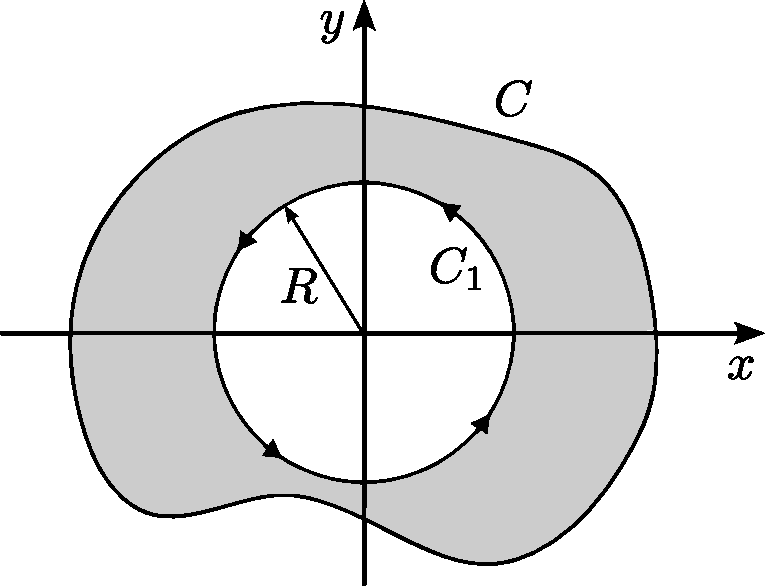
\includegraphics[width=0.25\textwidth]{figs/fig-10.pdf}
    %\caption{Ejercicio 4.}
%\end{wrapfigure}
\begin{question}  % Kreyszig example 6, pg 649
Sea $f(z) = (z - z_0)^m$, donde $m$ es un entero y $z_0$ una constante. Integrar la función sobre una trayectoria circular $C$ de radio $\rho$ con centro en $z_0$ en sentido antihorario. 
\end{question}


\begin{question}% H. Gross - 1.7.1(L) pg 3.
    Suponga que $\lim_{n \rightarrow \infty} a_n = L_1$ y $\lim_{n \rightarrow \infty} a_n = L_2$. Probar que $L_1 = L_2$.
\end{question}

\begin{question}  % H. Gross - 1.7.2(L) pg 3
Sea $f(z)$ definida por
\[ f(z) = 1 - 2 z + 3 z^2 -4 z^3 + \cdots = \sum_{n=0}^{\infty} (-1)^n (n + 1) z^n \]
\begin{enumerate}[a)]
    \item Encuentre el radio de convergencia de $f$.
    \item Calcule $f(\tfrac{i}{12})$ con una precisión dada por un disco de radio $0.001$.
    \item Calcule $f'(\tfrac{i}{12})$ con una precisión de un dígito decimal.
\end{enumerate}
\end{question}

\end{document}
